\section {Online $k$-Sketch Maintenance}\label{sec:online}
In the offline scenario, all the events are assumed 
to be available at the time of $k$-Sketch query processing. 
On the contrary, in the online scenario,
events arrive incrementally. 
Given an arrival event, our objective is to maintain the $k$-Sketch 
for each subject uptodate. Since events may arrive at a high speed, %arrival speed could be very high, 
such a maintenance step has to be done efficiently.  

Similar to the offline scenario, we maintain an index $WI$  to keep 
track of the top-$p$ streaks 
for all the possible streak lengths.
To handle a newly arrived event $e_s(t)$, a naive solution would first generate
all the streaks containing $e_s(t)$, (i.e. $W_s(t,w'), w'\in(1,t]$), and then
update $WI$ accordingly.
%For each streak, $WI$ is then updated accordingly. 
Last, Algorithm~\ref{algo:greedy} is invoked to re-compute the sketches. 
However, there are $t$ associated streaks for each new event $e_s(t)$. 
Examining all of them is too expensive to support real-time responses. 
Moreover, Algorithm~\ref{algo:greedy} runs in $O(k|\mathbb{N}_s|)$ 
time for each affected subject, which imposes further performance challenges. 

To achieve instant sketch maintenance, we propose two techniques: \emph{online streak pruning} and \emph{sketch update}. 
\emph{Online streak pruning} tries to reduce the number of streaks evaluated in generating ranked-streaks. 
After obtaining the ranked-streaks, we need to update the affected sketches.
As we shall see later, given a ranked-streak $N_s(t,w)$, 
not only the sketch of subject $s$ but also the sketches of other subjects could be affected. 
Although we provide a solution with a $(1-1/e)$ approximation in the offline scenario, 
maintaining sketches to achieve the same approximation ratio 
is difficult in the online scenario~\cite{Alonerbuch2003The,Awerbuch1996Making}. 
Therefore, we propose a $1/8$-approximate solution which updates a sketch in $O(k)$ time.
%sketch update solution which only takes $O(k)$ time.
% to perform the sketch update.

\begin{algorithm}[h]
\caption{Online $k$-Sketch Maintenence}\label{algo:online_overview}
\begin{algorithmic}[1]
\Require $e_s(t) \gets $ arrival event
\State $WI()$// top-$p$ streaks for each length
\State $\beta()$// smallest score in $WI$ for each streak length
\For{$w \in 1,...,t $}
\If{$W_s(t,w)$ can be added to $WI(w)$}
\State update $\beta(w)$, $J_s(w)$, compute $N_s(t,w)$ 
\State SketchUpdate($N_s(t,w)$)
\EndIf
%\State $P_s(w) = \frac{w}{w+1}W_s(t,w).\overline{v}+ min\{ \frac{t-w}{w+1}J_s(t-w), \frac{t-w}{t}J_s(1)\}$
\State compute $P_s(w)$
\State \bf{break} if $P_s(w)\leq \max\{\beta(w')|w < w' \leq t\}$
\EndFor
\end{algorithmic}
\end{algorithm}

Before we present \emph{online streak pruning} and \emph{sketch update}, 
Algorithm~\ref{algo:online_overview} first 
depicts the overview of our online solution against a new event $e_s(t)$. 
We iteratively examine 
streaks which contain $e_s(t)$ (i.e.,$W_s(t,w)$ in Line 3). 
Then we update the sketches which are affected by inserting $W_s(t,w)$ into $WI$ (Lines 4-7).
Before continuing to examine the next streak length $w$,
we compute the maximum score (i.e., $P_s(w)$) of all streaks which have not been evaluated. 
If $P_s(w)$ is smaller than all $\beta(w'), w' \in (w,t]$, 
we can safely stop processing since no further streaks could cause any sketches to change.

\subsection{Online Streak Pruning}
Since there are $t$ streaks associated with each new event $e_s(t)$, 
we wish to avoid enumerating all the possible cases. 
We achieve the online streak pruning by leveraging the online-streak bound denoted by $P_s(w)$, which
is the upper bound value among streaks with lengths greater than $w$. 
The value of $P_s(w)$ is stated as in the following theorem:

\begin{theorem}[Online-Streak Bound]
\label{thm:online_bound}
Let $W_s(t,1)$,$\ldots$, $W_s(t,w)$ be the $w$ streaks computed in Algorithm~\ref{algo:online_overview} containing event $e_s(t)$. Let $P_s(w)$ be:
\begin{equation}
	P_s(w) = \frac{w}{w+1}W_s(t,w).\overline{v}+ min\{\frac{t-w}{w+1}J_s(t-w), \frac{t-w}{t}J_s(1) \}
\end{equation}
Where $J_s(\cdot)$ is the visiting-streak bound.  Then $P_s(w)$ is the online-streak bound, i.e., $P_s(w) \geq \max\{W_s(t,x).\overline{v}| x \in (w,t]\}$.
\end{theorem}
\begin{proof}
First, $\forall x \in (w,t]$, we have: 
\begin{align*}
W_s(t,x).\overline{v} &= \frac{wW_s(t,w).\overline{v} + (x-w)W_s(t-w,x-w).\overline{v}}{x} \\
%& = \frac{wW_s(t,w).\overline{v}}{x} + \frac{(x-w)W_s(t-w,x-w).\overline{v}}{x} \\
& \leq \frac{wW_s(t,w).\overline{v}}{w+1} + \frac{(x-w)W_s(t-w,x-w).\overline{v}}{x}
\end{align*}

Note that $J_s(x-w) \geq W_s(t-w, x-w).\overline{v}$, and $yJ_s(y)$ monotonically increases with respect to $y$.
It follows that $(x-w)W_s(t-w,x-w).\overline{v}/{x} \leq (x-w)J_s(x-w)/{x} \leq (t-w)J_s(t-w)/(w+1)$.
%
On the other hand, $J_s(1)\geq W_s(\cdot,y).\overline{v}$, for any $y$. Therefore,
$(x-w)W_s(t-w,x-w).\overline{v}/{x} \leq (x-w)J_s(1)/x \leq (t-w)J_s(1)/t$.
Combining the above deductions, it follows that:
\begin{equation*}
\hspace{-4mm}\frac{(x-w)W_s(t-w,x-w).\overline{v}}{x} \leq min\{\frac{t-w}{w+1}J_s(t-w), \frac{t-w}{t}J_s(1) \}
\end{equation*}
which leads to Theorem~\ref{thm:online_bound}. 
\end{proof}

When $w$ is small, $\frac{t-w}{w+1}J_s(t-w)$ is too loose as $\frac{t-w}{w+1}$ is large. However, we can leverage $\frac{t-w}{t}J_s(1)$ to obtain a better bound. As $w$ increases, $\frac{t-w}{w+1}J_s(t-w)$ eventually becomes smaller than $\frac{t-w}{t}J_s(1)$. Thus, we can leverage $\frac{t-w}{w+1}J_s(t-w)$ to perform efficient pruning. 

%Using the same logic, we can derive bounds for other aggregate functions; these are listed in Section~\ref{sec:discussion}.

\subsection{Sketch Update}
\label{subsec:sketch_main}
Once we obtain a streak $W_s(t,w)$ which causes changes in the $WI(w)$, 
two kinds of sketch updates may occur. The first update is directly
on the sketch of $s$,
% is to update the sketch for subject $s$, 
which we refer to as \emph{active update}.
The second update is on the sketches for other subjects. 
%The second is to update the sketches for other subjects. 
This happens when some of their ranked-streaks become worse due to $W_s(t,w)$. 
We refer to this case as \emph{passive update}. If these 
updates are not properly handled, sketches maintained for those subjects 
are not able to obtain an approximation ratio on their qualities. 
We demonstrate the two types of updates in the following example.

\begin{figure}[h]
	\centering
    \begin{subfigure}[b]{0.453\textwidth}
        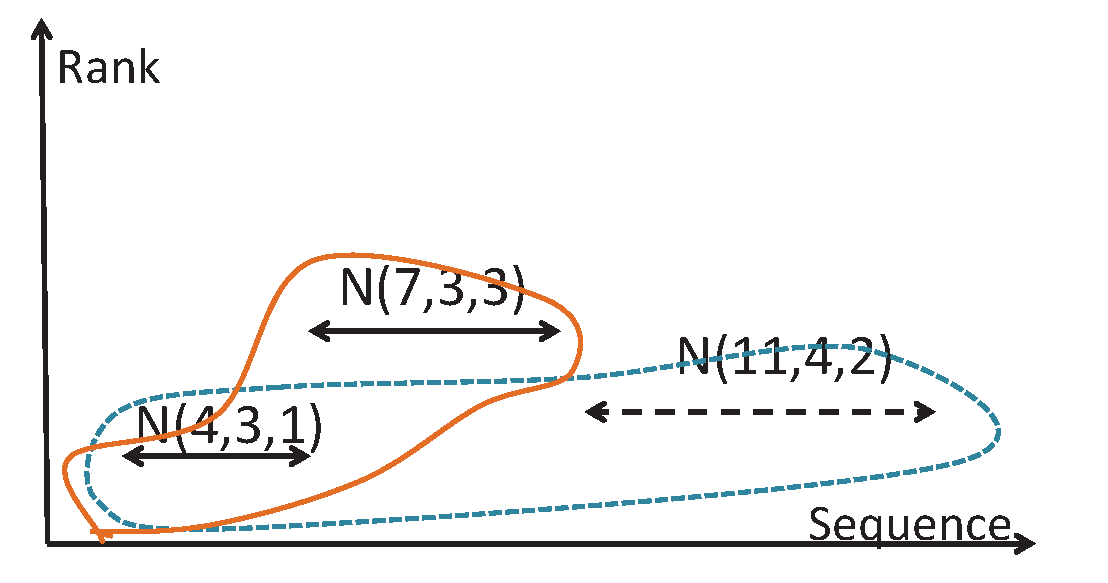
\includegraphics[width=\textwidth]{chpater4/active_update.eps}
        \caption{Active update cased by the new ranked-streak $N(11,4)$}
%        \label{fig:active_update}
    \end{subfigure}
    \begin{subfigure}[b]{0.45\textwidth}
        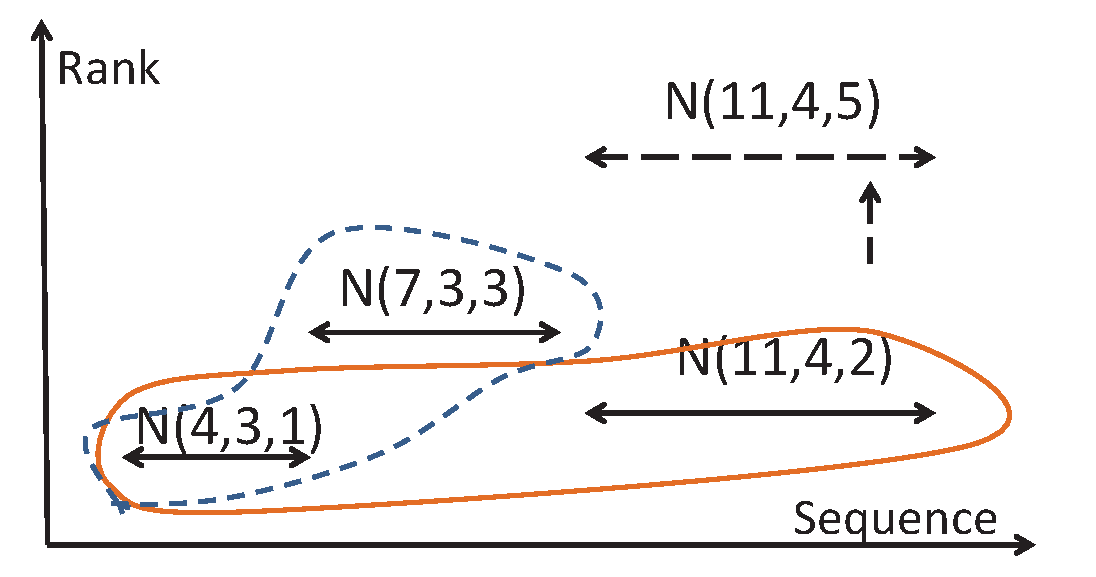
\includegraphics[width=\textwidth]{chpater4/passive_update.eps}
        \caption{Passive update cased by the existing ranked-streak $N(11,4)$ }
%        \label{fig:passive_update}
    \end{subfigure}
    \caption{The illustration of active updates and passive updates, the solid circle represents the original
    sketch, the dotted circle represents the updated sketch.}
    \label{fig:sketch_maintenance}
\end{figure}


\begin{example}
Suppose $k = 2$ and we maintain a $2$-Sketch for each subject. As shown in Figure~\ref{fig:sketch_maintenance}(a), 
when the ranked-streak $N(11,4)$ is generated, the maintained sketch is no longer the best. 
This is because replacing 
$N(7,3)$ would generate a better sketch. This process is referred as the \textbf{active update}.
In Figure~\ref{fig:sketch_maintenance}(b), $N(11,4)$ is pushed up due to the arrival of the event about another subject; as a result, the quality of the sketch drops. We name this process as the \textbf{passive update}. 
If passive update is not handled, the rank of $N(11,4)$ may continue to be pushing up and may eventually be greater than $p$, making the entire sketch invalid. Nevertheless, it is evident that when $N(11,4)$ degrades, replacing it with $N(7,3)$ would
result in a sketch with a better quality. 
\end{example}

A naive approach to handle these updates is to run Algorithm~\ref{algo:greedy} for each affected subject.
% whose sketches are affected.
This maintains a $(1-1/e)$-approximation ratio but incurs a high computational cost. 
In order to support efficient updates, we make a trade-off between 
the quality of the sketch and the update efficiency by 
providing a $1/8$-approximate solution with 
only $O(k)$ ranked-streaks being accessed for each affected subject. 

In particular, we maintain two size-$k$ sets $S_1$ and $S_2$. 
$S_1$ maintains the $k$ best ranked-streaks which collectively cover most
events whereas $S_2$ maintains $k$ ranked-streaks with best ranks. 
When performing an active update for a streak $N_s(t,w)$, 
we check if $N_s(t,w)$ could replace any ranked-streak in $S_1$ 
to generate a better cover. Meanwhile, we select the new 
$k$ best ranked-streaks into $S_2$. 
After $S_1$ and $S_2$ are updated, 
we perform the greedy selection from $S_1 \cup S_2$.
During a passive update, $S_1$ is not affected. We simply update $S_2$ to be the new $k$ best ranked-streaks. 
Afterwards, the new sketch is obtained by performing a greedy selection from $S_1 \cup S_2$. Algorithm~\ref{algo:online_update} presents both the active and passive updates. 
%
%Let scoring function $C(S)$ be the cardinality of sequences covered by all elements in $S$, $R_i$ be the
%all news candidates of object $i$, then our algorithm works as follows: 
\begin{algorithm}
\caption{SketchUpdate}\label{algo:online_update}
\begin{algorithmic} [1]
\Require $N_s(t,w)$
\State \textbf{Active update for the subject $s$}
\State $S_1$:  $k$ ranked-streaks with best cover
\State $S_2$:  $k$ ranked-streaks with best ranks 
\State $N^* \gets \argmax_{N \in S_1}C(S_1 \cup N_s(t,w) \setminus N)$
\If{$C(S_1) < C(S_1 \cup N_s(t,w) \setminus N^*)$}
\State $S_1 \gets S_1 \cup N_s(t,w) \setminus N^*$
\EndIf
\State $S_2 \gets$ new $k$ ranked-streaks with best ranks 
\State $S \gets greedy(S_1 \cup S_2 )$
\\\hrulefill
\State \textbf{Passive update for an affecting subject $s'$}
\State $S_2 \gets$ new $k$ ranked-streaks with best ranks for $s'$
\State $S \gets greedy(S_1 \cup S_2)$
\end{algorithmic}
\end{algorithm}
  
%\begin{algorithm}
%\caption{Passive Update for Subject $s$}
%\begin{algorithmic} [1]
%\end{algorithmic}
%\label{algo:online_passive_update}
%\end{algorithm}

We state the quality of our sketch update strategy in the
following theorem:
%
%Given our sketch update strategies,
%we are now ready to prove the approximation ratio for the maintained sketches. 

\begin{theorem}[Approximation Ratio for Sketch Update]
\label{thm:online_quality}
Each sketch maintained by Algorithms~\ref{algo:online_overview}
achieves an at least $1/8$-approximation to the optimal solution.
\end{theorem}

\begin{proof}
First, we observe that $S_2$ always keeps the ranked-streaks with optimal ranks. 
Second, we note that $S_1$ maintains the streaks with $1/4$-approximate coverage as shown in~\cite{Saha2009On}.

Let $OPT_C$ be the optimal $k$ streaks that best covers $s$'s history; Let $C()$ be the number of events a set of streaks cover. Similarly, let $OPT_R$ be the optimal $k$ streaks with highest ranks; Let $R()$ be the 
summation of ranks of all members in a ranked-streak set. Let $S^*_s$ be the optimal sketch of subject $s$. Intuitively, we have the following: 
\begin{equation*} 
g'(S^*_s) \leq \eta_1 C(OPT_C) + \eta_2 R(OPT_R)
\end{equation*}
Since $C(S_1) \geq 1/4 C(OPT_C)$ and $R(S_2) = R(OPT_R)$, we have the following:
\begin{equation*}
\begin{split}
\eta_1 C(S_1) + \eta_2 R(S_2) & \geq 1/4 * \eta_1 C(OPT_C) + \eta_2 R(OPT_R) \\
& \geq 1/4 g'(S^*_s)
\end{split}
\end{equation*}
which implies $\max\{\eta_1 C(S_1), \eta_2 R(S_2)\} \geq 1/8 g( S^*_s)$. 
As $g'(S_1) \geq \eta_1 C(S_1)$ and $g'(S_2) > \eta_2 R(S_2)$, it leads to:
\begin{equation*}
\max\{g'(S_1), g'(S_2)\} > 1/8  g'(S^*_s)
\end{equation*}
Let $SK_s$ be one of the sketch maintained by Algorithms~\ref{algo:online_update},
since the greedy algorithm is run on $S_1 \cup S_2$, 
$g'(SK_s) \geq max(g'(S_1), g'(S_2)) \geq 1/8 g'(S^*_s)$.
As a result, our algorithm always ensures at least $1/8$-approximation for each sketch.
\end{proof}

%We model the news selection problem as follows: Given a event
%$e$, let $C$ denote the news candidates derived from $e$. Each news
%candidate is of the form $\langle sid, w, t, r\rangle$, where $sid$ is the
%identifier of subject, $w$ is the
%length of this news candidate, $t$ is the end time this candidate and $r$
%is the rank of this news candidate w.r.t other news candidates with 
%similar window size. 
%
%Let $R(sid, T)$ be the set of news that has been reported of subject $sid$ prior to
%the time sequence $T$, i.e., $R(sid,T)={n| n.sid = sid, n.t < T}$. When no ambiguity, 
%we use $R(T)$ for short.
%In order to maintain the quality of the news reported for a subject, we 
%wish to fulfill the following two criteria:
%\begin{enumerate}
%\item the news candidates in $R(T)$ needs to cover the most events in the subject's history
%\item the ranks of the news in $R(T)$ needs to be as low as possible
%\end{enumerate}
%
%The first criteria tends to provide the comprehensive news which covers the subject's
%past history, the second criteria tends to select the most quality news out of the news candidate.
%
%Therefore, given a set of news, we define a evaluation function as follows:
%\begin{equation}
%	F(X) =  \Sigma_{n \in X}(n.w * n.r)
%\end{equation}
%
%In order to consider both criteria, we insert \emph{unit news candidate} of form $u(t_i)=\langle sid,1,t_i,R\rangle$
%,where $R$ is the maximum rank that considered to be meaningful. For $R(T)$, we insert $T$ unit
%news candidates into it, so that our problem is defined to be a set cover: Given $R(T) = {S_1,S_2,...,S_k}$ where 
%each $S_i$ is a (unit) news candidate. Consider a ground set $G = \{1,...,T\}$. Our objective is to find a set $X \subseteq R$ 
%such that $\cup_{x_i \in X} [x_i.t-w, x_i.t] \supseteq G$ and $F(X)$ is minimized.

%The online version of the problem is that, given two sets $R(T-1)$ and $C(T)$ where $R(T-1)$ is the reported
%news and $C(T)$ is the online derived news candidates. Our objective is to find a subset $C' \subseteq C$ such that
%$\cup_{x_i \in (R \cup C')}[x_i.t-w, x_i.t] \supseteq (G \cup T+1)$ and $F(R \cup C')$ is minimized.
%
%It is easy to see that, the online version of the problem can be used for new events reporting, while
%the offline version of the problem can be used for history analysis of subjects.


%\subsubsection{Optimal Method for Offline Problem}
%The offline method is clearly a weighted vertex cover problem which is known to be NP-hard.
%For this problem, the optimal solution can be achieved via dynamic programming. Let $M[i][X]$
%be the \emph{optimal} value for using sets $S_1,S_2,...,S_i$ in set $R$ covering sets $X$, 
%we have the following relationship:
%\begin{equation}
%M[i][X] = min\{M[i-1][X-S_i] + S_i.r, M[i-1][X]\}
%\end{equation}
%
%Based on the equation, the optimal dynamic programming algorithm takes $O(k\times 2 ^{t})$ space
%and time. Although by some careful design, the space is able to reduce to $O(2^{t})$, both the 
%space and time complexity are not feasible for relatively large number of news detection. 
%
%We tackle the high complexity by first providing a branch-and-bound search for dynamic programming.
%Our main observation is that there exists dominance relationship between news events.

%\section{View Based Query Processing}
%In this section, we propose a view based query processing strategy to 
%timely process each arriving event. The notations used in the remaining
%of the paper is shown in Table~\ref{tbl:notations}.
%
%
%
%In our framework, processing a new 
%event $e=(id,V,s)$ consists of three phases. First, the event window $W_1$,...,$W_{s}$
%are derived. Second, for each event window $W_w$, its corresponding news candidate is
%formed by $N_w=\langle id, w, f_a(W_w), r \rangle$. Third, each $N_w$ is assessed by
%the scoring function $S$ and filtered by the threshold $\eta$.
%
%The main bottleneck of the processing is on second step where each $W_w$ needs to find 
%its rank among \textbf{all} other window events with the same size. If there are $s$ subjects
%in the application history, with each subjects has $m$ events, there are $O(ms)$ comparisons
%required to find $f_a(W_w)$'s rank.   
%
%
%Continuous Aggregation Detection for a new event $e=(o,a,v,t)$ entails 
%two phases. The first phase is to generate all possible event windows containing $e$. This results in $|t|$ new event windows. The second phase is 
%to verify that any of these $t$ new event windows are belong to the corresponding top-$k$ list. 
%
%To efficiently accomplish the second phase, the \emph{Top-$k$ Event Window Index} $H$ is necessary. Basically, for each window size $w$, $H_w$ maintains the top-$k$ lists of window event of size $w$. Given the set of existing events, $H$ can be built in off-line.
%
%A brute-force approach is thus as follows: \textbf{off-line phase}: For each $w$, generate the all possible event window of size $w$. Create $H_w$ with the top-$k$ event windows of size $w$. \textbf{on-line phase}: For newly arrived event $e$, for each $w$, compute the event window of size $w$ containing $e$.  Check for each $w$, report $e$ and $w$ if the event window is in $H_w$. 
%
%A simple analysis reveals the inefficiencies in the brute-force approach. In off-line phase, suppose there are $n$ objects, each with $w$ events, there are $\Theta(nw^2)$ event windows. Then computing the top-$k$ events is at least $\Theta(log(k)nw^2)$. In online phase, generating all $w$ event windows takes $\Theta(w)$ while checking for top-$k$ existence takes $\Theta(log(k))$. So the total complexity for a single event query is $\Theta(log(k)w)$.
%
%The inefficiencies with brute-force approach lies in: in off-line phase, it compute \textbf{every} window sizes for \textbf{every} object to generate the index. In on-line phase, it checks for event window of \textbf{every} size to report the full results. We thus devise several optimization to reduce the overhead. In the following sections, we will describe our techniques in two aspects: the index construction and query processing.

